\chapter{3D proto-object based saliency}
\label{sec:saliency}
\chaptermark{3D visual saliency}

\section{Introduction}

The brain receives large amounts of visual information that it must make sense of in real-time. Processing the entire visual field with the same level of detail present at the fovea would be an exceedingly complex and costly task requiring much greater computational resources than are available to the brain~\citep{Tsotsos90}. As a result, primates select only the most relevant information and discard the rest, a process known as selective visual attention.
%
\comment{Visual attention is controlled by both bottom-up and top-down mechanisms, which interact to influence the organism's behavior~\citep{Yarbus67}. Bottom-up attention is involuntary and signal-driven, largely due to the fact that some stimuli are more conspicuous and able to stand out from their surroundings. Top-down attention is task-dependent, and can take into account semantic information such as the familiarity or interestingness of an object, which biases the organism's attention based on its internal state or goals.}
%
Many models of visual attention are constructed with a bottom-up architecture and rely on local contrast in low-level features such as intensity, color, orientation, or motion. Biologically-plausible center-surround differences across different feature channels of an input image can be used to compute a ``saliency map'' whose maxima indicate where selective attention is deployed~\citep{Koch_Ullman85,Niebur_Koch96b,Itti_etal98a}.

However, there is both psychophysical~\citep{Einhauser_etal08a} and neurophysiological~\citep{Zhou_etal00, Qiu_etal07} evidence that attention relies not only on these simple image features, but also on the perceptual organization of the visual scene into tentative objects, or proto-objects~\citep{Rensink00a}. Biologically-inspired models of proto-object based saliency have been proposed that take into account these recent findings~\citep{Craft_etal07,Mihalas_etal11b,Russell_etal14}. These models include border-ownership selective cells (referred to as border-ownership cells in the following) and grouping cells, which interact to achieve figure-ground segmentation of the image into proto-objects (figures) and the background (ground).

Border-ownership cells have been found in primate visual cortex, with the majority of neurons in area V2 having this property. These cells signal in their neural activity the one-sided assignment of an object border to the region perceived as figure~\citep{Zhou_etal00}. Border-ownership cells are also modulated by attentional influences~\citep{Qiu_etal07}. Grouping cells integrate global context information about proto-objects in the scene according to Gestalt principles such as closure, continuity, convexity \etc Importantly, grouping cells act at intermediate stages of vision and do not require higher-level information about object identity, semantic knowledge \etc They send feedback to border-ownership cells \via fast white matter projections, which bias the activity of border-ownership cells to reflect the correct figure-ground segmentation of proto-objects. In this framework, visual saliency is a function of grouping cell activity, which represents the size and location of proto-objects within the image.

Border-ownership cells have been shown to respond to figure edges defined by a variety of image features, \eg luminance edges, color edges \etc When no monocular edge information is present (\ie when the figures are defined by random dot stereograms using only binocular disparity), border-ownership selectivity is also imparted by stereoscopic edges~\citep{Qiu_vonderHeydt05}. Critically, their response to these different figural cues is typically the same in the two-dimensional (2D) and three-dimensional (3D) cases -- the preferred side-of-figure of border-ownership cells is consistent for all cues that define the figure. The activity of border-ownership cells thus provides an interpretation of the visual scene in terms of depth-ordered surfaces that correspond to objects in 3D space.
%
\comment{In a separate line of work, it has been shown that surface representations play a key role in intermediate-level vision, and that visual attention can be deployed at the level of perceptual surfaces~\citep[][for a model of attention to surfaces see Hu \etal 2015]{He_Nakayama92,He_Nakayama95}.\nocite{Hu_etal15a}}
%
Despite these experimental observations, current models of border ownership do not explicitly use depth information and do not address how traditional 2D Gestalt cues interact with depth cues during the figure-ground segmentation process. An exception is a study by~\cite{Mishra_etal12} who used computer vision methods to compute border ownership from low-level depth information and then performed object segmentation in natural images.

Even though in recent years stereoscopic 3D content has become increasingly prevalent, \eg in the viewing of entertainment programs in cinemas and homes, little is known about how visual attention is deployed within 3D environments. It is thus important to understand how humans allocate their attention when viewing natural images and videos in 3D~\citep{LeCallet_Niebur13}. Binocular disparity cues, which can be used to generate strong depth percepts, have been shown to alter different aspects of eye movements when participants viewed 3D images~\citep{Jansen_etal09} and videos~\citep{Huynh_Schiatti11}. Only recently have 3D eye tracking datasets been made available which can be used to compare human eye movements with predictions of attentional models. The availability of these datasets and the recent explosion in new 3D content makes it possible to design computational models of 3D saliency and evaluate their performance objectively.

\comment{The goals of our research are (1)~to extend a proto-object based saliency model~\citep{Russell_etal14} to include depth information, and (2)~to evaluate its performance in perceptual saliency prediction. We show that combining 2D Gestalt cues with depth cues improves the performance of our model on three different 3D eye tracking datasets. In the model, depth information along with other 2D features biases grouping cell activity, which then interacts with border-ownership cells to represent proto-objects, the tentative objects within the scene. These proto-objects are a first step in figure-ground segmentation of the image, and also give an indication of the salient points within the image. We evaluate the proto-object saliency maps produced by our model against ground truth data in the form of human eye fixations using a battery of different metrics.}

\section{Related Work}

\subsection{Models of 3D visual attention}

Compared to the number of models that have been proposed for 2D visual saliency, relatively few attempts have been made to study how visual attention is deployed within 3D environments. Existing models of 3D visual attention often compute a 2D saliency map which is then combined with the depth information to produce a new saliency map. These models fall into three categories~\citep{Wang_etal13} based on how the depth information is used: stereovision models, depth-weighting models, and depth-saliency models. For a comprehensive review of 3D visual attention models, see~\cite{Wang_etal13,Ma_Hang15}.

While the depth-weighting and depth-saliency models assume that a depth map has been computed, without specifying how, stereovision models explicitly implement the computation of depth information from the left and right views of the scene, thus replicating the human visual system's stereoscopic perception. An example of this is a study by~\cite{Bruce_Tsotsos05}, which extended a 2D selective tuning model of attention to also incorporate binocular information. However, no quantitative assessment of this model was performed.

Depth-weighting models use a base 2D saliency model (computed using one of the existing methods) and then multiplicatively weight the resulting saliency map with the depth information. Regions that are closer to the observer obtain higher weights, corresponding to greater combined saliency. In a model developed by~\cite{Lang_etal12}, novel depth priors are learned from a training portion of the data, and these are then combined with the output of a 2D saliency model either using pixel-wise addition or multiplication. With these depth priors, the authors find an increase of performance by 6-7\% on their dataset compared to the base 2D model without depth information.

Depth-saliency models come in two flavors. In one, both a depth saliency map, obtained from depth alone, and a more traditional saliency map, obtained from 2D information alone, are computed. The two maps are then linearly combined to generate the final saliency map.~\cite{Wang_etal13} determine depth saliency in a separate experiment involving synthetic stereoscopic stimuli, which allows them to reduce the influence of monocular depth cues, as well as control for the depth of objects and the background. With their experimental results, they propose a probabilistic model of depth saliency, where the probability of a point being fixated in 3D space is related to the magnitude of center-surround differences in depth contrast. Linearly combining these two saliency maps in a 1:1 ratio (50\% weight each for 2D features and depth information) results in better performance on their dataset. In the second type of depth-saliency models, depth information is treated as an additional feature channel, on the same footing as intensity, color, orientation \etc The final saliency map is then a function of depth as well as of these other features~\citep{Ouerhani_etal00,Jost_etal04,Hugli_etal05}.

Our approach falls in the latter class of depth-saliency models, where all image features, including depth, interact through linear combination resulting in the final saliency map. Our model is completely integrated -- depth information is treated as another cue which interacts with 2D Gestalt cues to influence figure-ground assignment of proto-objects within the scene. This agrees with anatomical and neurophysiological data that show that disparity selective cells, which are important for encoding stereoscopic depth information, are found in the same early cortical areas as neurons representing other features used in typical saliency models, like color and orientation~\citep{Hubel_Wiesel62,Poggio_etal88b}. Different
from previous models~\citep{Ouerhani_etal00,Jost_etal04,Hugli_etal05}, our model is not only based on basic image features (like color, intensity \etc) but it includes elements of perceptual organization, in particular proto-objects. The model is an extension of a previously described 2D model~\citep{Russell_etal14} and is constructed by including depth information as an additional feature. All features are used to determine proto-object based saliency. We tested our model on the three 3D eye tracking datasets listed in the next section, and we compared results with and without the added depth information.

\subsection{3D eyetracking datasets}

A common method for evaluating the quality of computational models of visual attention is to compare their performance in the prediction of human eye movements. Since its introduction by~\cite{Parkhurst_etal02a}, this method has been used in a large number of studies, both for static and dynamic scenes (video) and both for human and non-human primates~\citep[for a recent review see][]{Borji_Itti13}. Nearly all of this work has been limited, however, to 2D scenes.

In order to evaluate 3D attention models, eye tracking data on a variety of visual scenes have to be collected. We use datasets of natural images consisting of color images and associated depth maps along with human fixations for each image.  Predictions of saliency maps for eye movements can then be compared to the ground truth fixation data using various metrics. Below, three such publicly available datasets are described. Figure~\ref{Fig:Results} shows one example of the data available from each of them. 

\begin{figure}[t]
\centering
\includegraphics[width=\textwidth]{3D-Saliency/figs/Results_Fig.eps}
\makeatletter
\let\@currsize\normalsize
\caption[Examples of 3D image data used and saliency maps obtained]{Examples of data used and results obtained. Columns (left to right) show one example each of the original image with its corresponding depth map, fixation map, our saliency model without ($S$) and with ($S_d$) depth information for the three 3D eye tracking datasets: a) NUS-3D. b) Gaze-3D. c) NCTU-3D.}
\label{Fig:Results}
\end{figure}

The NUS-3D dataset~\citep{Lang_etal12} contains 600 RGB and depth image pairs, each with a resolution of $640\times480$ pixels. The images show various scenes around the National University of Singapore (NUS) campus and were collected with a Microsoft Kinect camera, which is capable of recording both RGB and depth images. The Kinect depth sensor is affected by ambient lighting and has a depth range of only about 4~m, which restricts the types of scenes it can accurately capture. The images were presented to 80 participants and each participant's eye tracking data was captured in both 2D and 3D free-viewing experiments. The 3D stimuli were generated by virtual view synthesis~\cite[see][for details]{Lang_etal12} but the synthesized 3D images are not available to the public. Only the raw and smoothed depth maps from the Kinect as well as the fixation density
maps for the 2D and 3D viewing conditions are available.

The Gaze-3D dataset~\citep{Wang_etal13} consists of 18 stereoscopic images, along with their associated disparity maps and perceived depth maps~\cite[perceived depth is computed from raw disparity by taking into account viewing distance and display properties; see][for details]{Wang_etal13}. The ground truth disparity maps were calculated from separate left and right image views using an optical flow method~\citep{Werlberger_etal09}. The images come from the Middlebury 2005/2006 stereo image dataset~\citep{Scharstein_Pal07} and the IVC 3D image dataset~\citep{Urvoy_etal12}. The dataset also contains raw eye tracking data for both the left and right eyes, as well as processed fixation density maps from a total of 35 participants. The images are high resolution ($1300\times1080$ pixels for the Middlebury subset and $1920\times1080$ pixels for the IVC subset) and have relatively accurate depth information. A limitation is the small number of images in the dataset.

The NCTU-3D dataset~\citep{Ma_Hang15} consists of 475 2D images with a resolution of $1920\times1080$ pixels along with their corresponding depth maps and eye tracking data. The eye tracking data is in the form of fixation density maps and binary fixation maps. The images in the dataset were collected from randomly selected frames extracted from 11 different sequences of 3D videos from either Youtube (youtube.com) or 3dtv (3dtv.at). The depth maps were generated from left and right eye views using Depth Estimation Reference Software (DERS; version 5.0). A total of 16 participants freely viewed the videos in 3D.

\section{Methods}

\subsection{Model}

Our approach is based on the proto-object based saliency model proposed by~\cite{Russell_etal14}. In the model, grouping cells group visual features into proto-objects that are characterized by their locations and spatial scales. The large annular receptive fields of the grouping cells enforce the Gestalt principles of closure and convexity, which in turn biases the activity of proto-objects towards the center of objects. Proto-objects are then a means to organize the scene into separate figures as well as the background. The grouping mechanism operates on multiple feature channels and incorporates competition between proto-objects of similar size and feature type. The model explains the development of border-ownership findings in primate cortex~\citep{Craft_etal07,Zhou_etal00}. Given that human eye movements tend to fall predominantly on objects~\citep[][ but see~\cite{Borji_etal13} for a different view]{Einhauser_etal08a}, which are often closed and convex, the locations of proto-objects are also assumed to correlate with the salient points within the image. For a full description of the original model, we refer the reader to~\cite{Russell_etal14}.

We extend this model to include depth information. Since some images have border artifacts, all images are cropped to avoid spurious model responses at the borders. To achieve scale invariance, we create an image pyramid spanning 8-10 octaves (depending on the size of the image) by successively down-sampling the input image in steps of 2. We use a minimum cut-off image size of $3\times 3$ pixels, such that pyramid levels that would reduce the image size below $3\times 3$ pixels are not included in our model. All operations are applied independently to each feature and at each level of the feature pyramids, except for when the scales and features are combined to obtain the final saliency map. Each layer of the network represents the neural activity of an array of neurons which tile the visual scene and which are propagated to other layers in the network through feedforward connections. The receptive fields of neurons are described by different correlation kernels, and the image input to each neuron in the model is calculated using the correlation operation. The model was implemented using MATLAB (Mathworks, Natick, MA). A model overview is shown in Figure~\ref{Fig:Model}.

\begin{figure}[t]
\centering
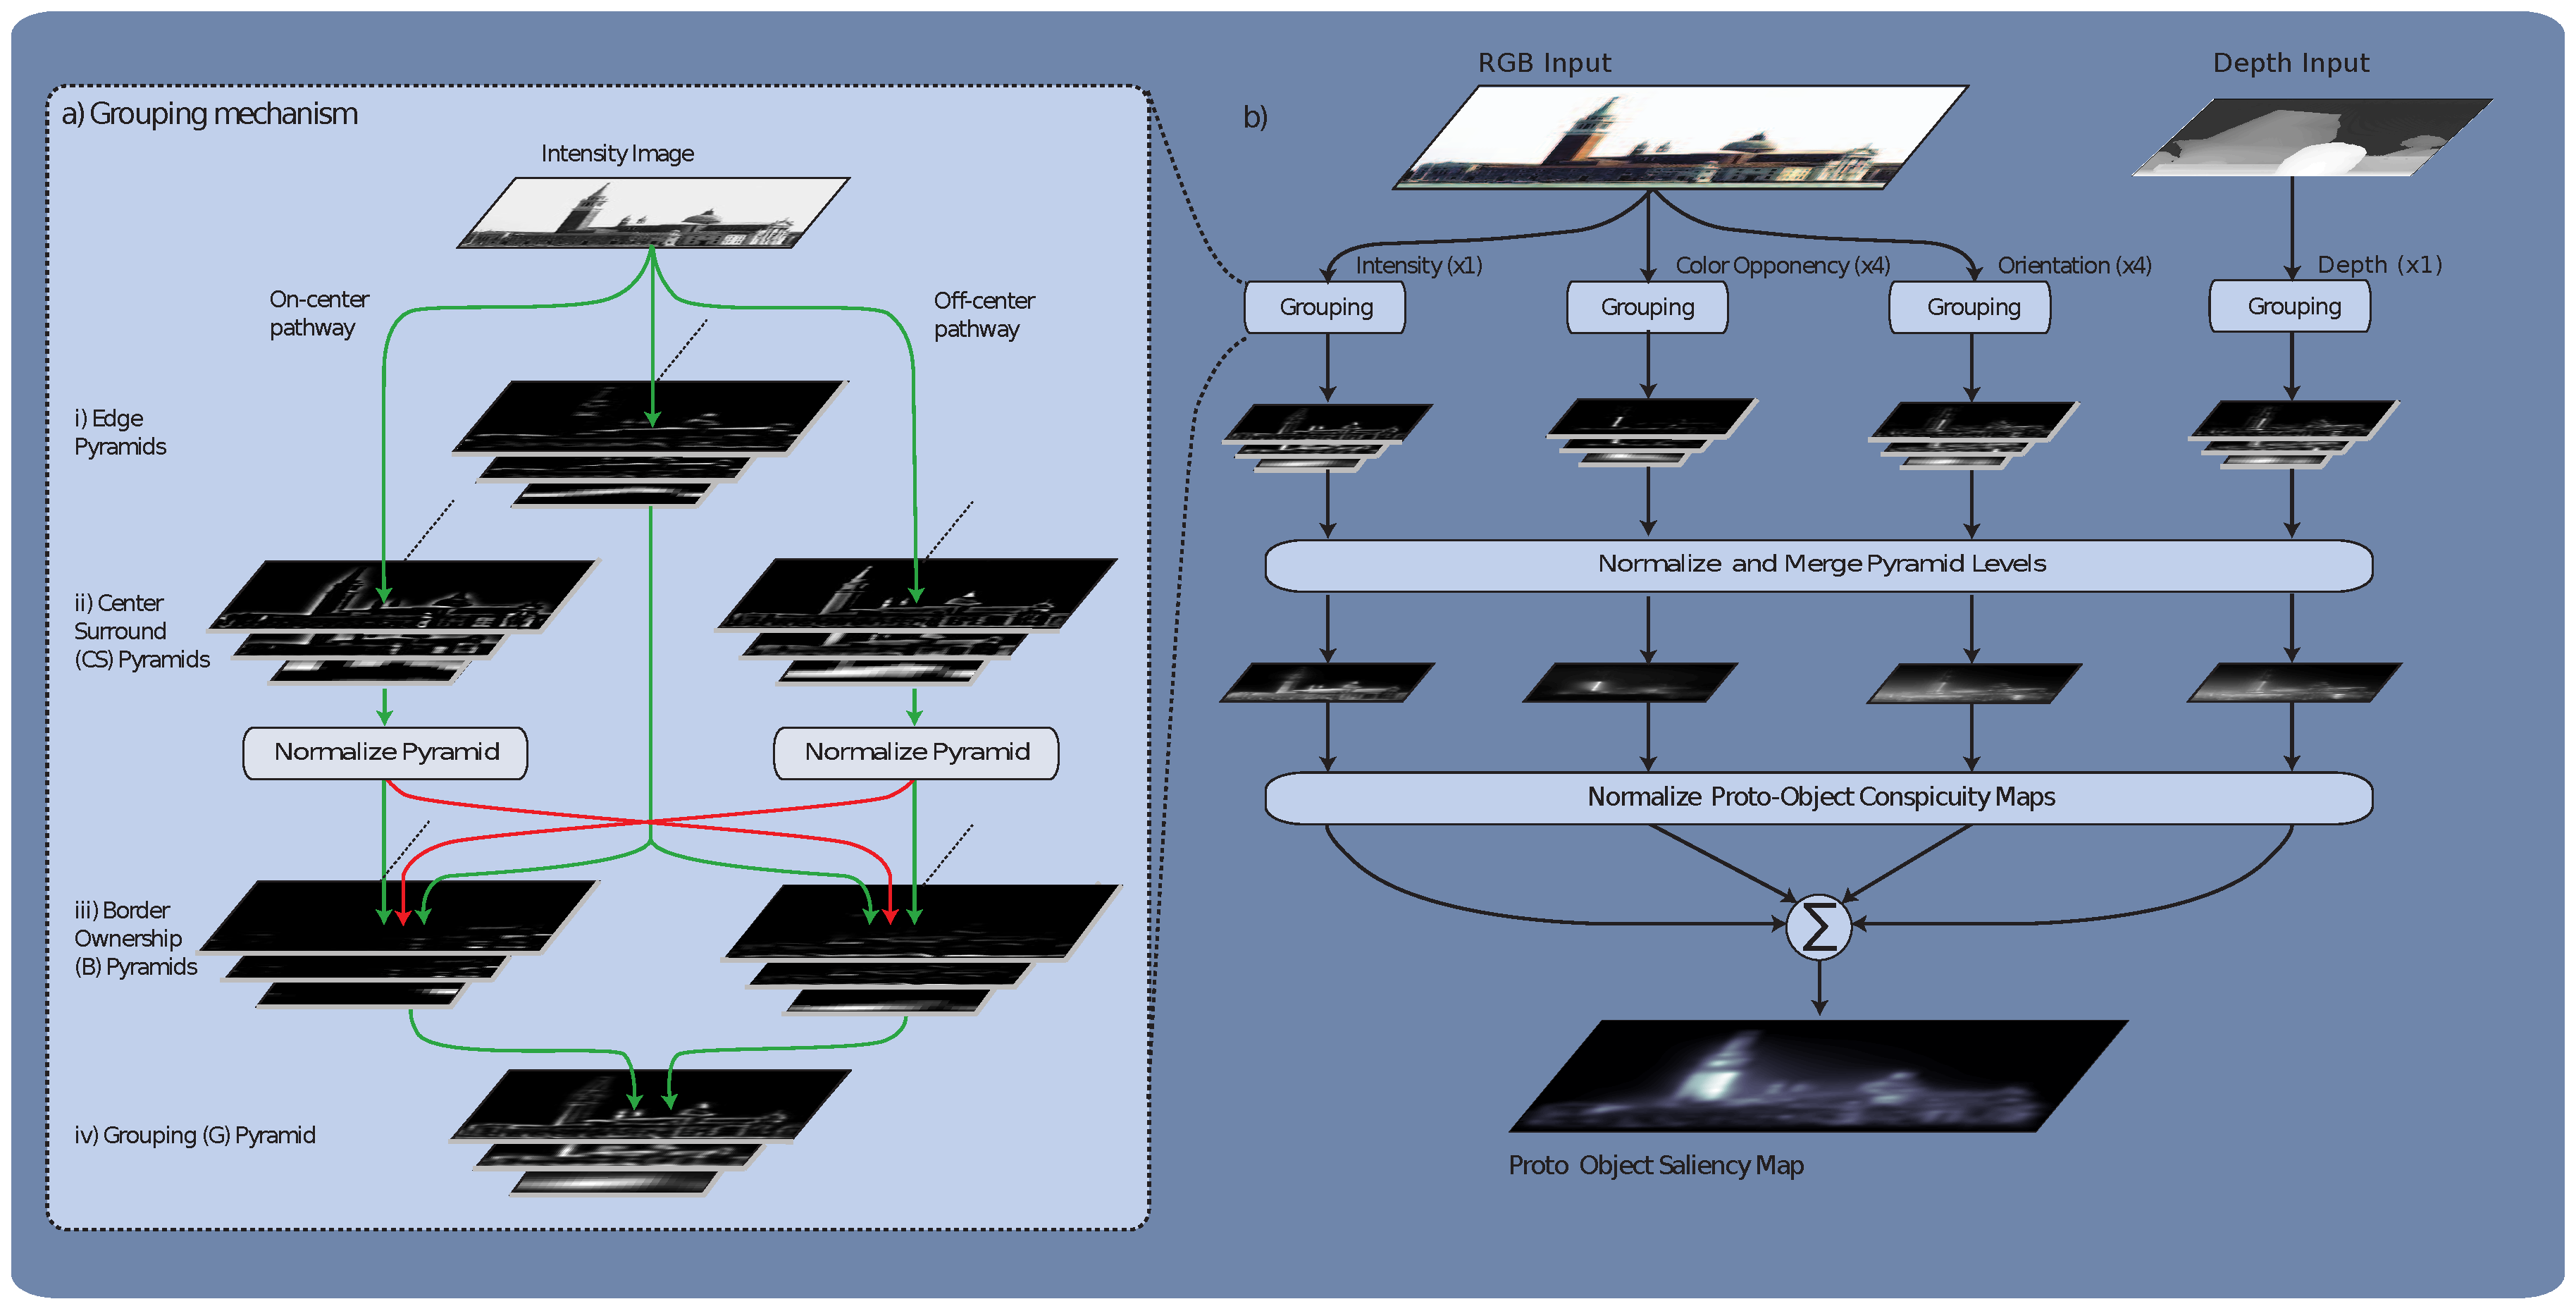
\includegraphics[width=\textwidth]{3D-Saliency/figs/DepthSaliency_new1.eps}
\makeatletter
\let\@currsize\normalsize
\caption[Proto-object saliency model with added depth information]{Proto-object saliency model with added depth information. The depth map is represented by the image at the top, far right, and the 2D image is to its left. Based on Figure~5 of~\cite{Russell_etal14}.}
\label{Fig:Model}
\end{figure}

In this chapter, we will refer to the saliency map generated by the original 2D model without depth information as $S$, and to the saliency model generated by our new model, which incorporates depth information as $S_d$. To compute $S$, the model accepts an input RGB image and decomposes it into different feature channels: one intensity channel, four color-opponency channels, and four orientation channels. Rather than providing ``raw'' stereoscopic disparity information in the form of different images to the two eyes (or retinae), we assume that the transformation from disparity information to depth has been performed at the input level to our model. There is well-known neuronal circuitry that transforms stereoscopic disparity into depth information~\cite[\eg][]{Poggio_Poggio84} and the explicit representation of depth is more appropriate for the intermediate-vision conceptual level of our proto-object based model than the ``raw'' representation in terms of binocular disparity. Therefore, to compute $S_d$, we add an additional depth feature channel obtained from the input depth image. Within each feature channel, we perform edge filtering (using oriented Gabor filters at 4 orientations) to obtain the location of proto-object borders. In order to perform feedforward computation of figure-ground segregation, we employ a center-surround mechanism, similar to that used by~\cite{Itti_etal98a}; such mechanisms have been observed at multiple stages in the brain, including retina, lateral geniculate nucleus, and cortex (\ibid). This center-surround mechanism provides context information about proto-objects, and biases the activity of border-ownership cells with preferred directions that match the location of the figure.

For the 2D features used in our model, the center-surround mechanism is symmetric with respect to figure-ground contrast polarity (\eg light figures on dark backgrounds or dark figures on light background result in the same net salience contribution). In contrast, for the depth channel we compute the center-surround differences in an asymmetrical manner, consistent with the kind of information provided by stereoscopic depth. While most feature differences across a contour are not predictive about which of its sides is the foreground\footnote{Exceptions are T-junctions~\citep{Heitger_vonderHeydt93} and extremal edges~\citep{Palmer_Ghose08,Ramenahalli_etal11a,Ramenahalli_etal12a,Ramenahalli_etal14a} both of which are local cues that provide information about edge polarity.\label{EEfootnote}}, stereoscopic depth (disparity) provides nearly unambiguous information about which side of the border is closer to the observer. This side ``owns'' the object border when considered in a depth ordering sense and is part of the foreground. Physiological data show that the responses of border-ownership cells to disparity differences across a figure edge are in agreement with this observation~\citep{Zhou_etal00,Qiu_vonderHeydt05}. Therefore, in our model near \vs far depth differences bias the activity of border-ownership cells such that the near side is more likely to be classified as the foreground object. Integrating depth information into the representation of an object by its contours is a critical difference between our model and other depth saliency models which directly combine depth feature information with 2D information, without taking into account perceptual grouping effects~\cite[\eg][]{Ouerhani_etal00,Jost_etal04,Hugli_etal05}. By modeling the response of border-ownership cells to depth edges, we enforce an additional constraint on how depth information is to be combined with 2D information in order to produce proto-objects and the resulting salient points of the image.

Each channel is processed independently of the others by the same grouping mechanism, and then combined through a series of normalization operators, which allow for competition between proto-objects of similar scale and feature. The final feature map is obtained by scaling each map to a common scale (approximately the middle level of the image pyramid), and then performing a pixel-wise addition across scales. The different feature conspicuity maps are then normalized again and linearly combined with equal weights to form the proto-object saliency map $S$. When depth information is used, we use a linear combination of 80\% 2D features, split equally among intensity, color, and orientation, and 20\% depth features to form the depth-added proto-object saliency map $S_d$. Obviously, this fraction can be modified but we found that results do not critically depend on its choice (see also the \hyperref[sec:saliency_discussion]{Discussion}).

\subsection{Evaluation metrics}

We evaluate the performance of our model by comparing our generated saliency maps with ground truth data in the form of human eye fixations. Different from many other studies, we tested our model with a whole battery of metrics that were {\em not} necessarily chosen to give good results. We did this in order to provide a more diverse picture of the model's overall performance. ~\cite{Riche_etal13} have suggested that at least three different metrics are needed to fairly evaluate a given model. To ensure that our results do not depend on the use of a specific evaluation method, we use a battery of commonly used saliency metrics: area under the curve (AUC), Pearson's linear cross-correlation (PLCC), normalized scanpath saliency (NSS), similarity (SIM), earth-mover's distance (EMD), and the Kullback-Leibler divergence (KLD). For a recent review see~\cite{Riche_etal13}, the following is a brief description of the metrics.

KLD, EMD, PLCC, and SIM are distribution-based metrics that measure the similarity/dissimilarity between two distributions (in our case, between the distribution of human eye fixations and of the salient points as predicted by the model). Larger values of KLD and EMD indicate a larger overall difference between the two distributions, while a value of zero indicates that the two distributions are not systematically different from each other. PLCC and SIM are bounded values, where a value of unity indicates that the two distributions are identical, while a value of zero indicates that the distributions are completely uncorrelated (PLCC can also be negative, indicating a negative correlation between the two distributions). AUC is a location-based metric, a measure borrowed from signal-detection theory. An equal number of fixated and random pixels are first chosen from the saliency map. A threshold is then applied to the saliency map, which acts as a classifier, with all saliency points above threshold considered ''fixated,'' and all saliency points below threshold considered ''background.'' For each threshold value, we can then determine a true positive rate and a false positive rate based on the ground truth eye fixation map, which allows us to generate a Receiver-Operator Characteristic (ROC) curve and calculate the corresponding Area Under the Curve (AUC) metric. An ideal score is unity while a random classification gives a score of 0.5 and systematic mis-classifications result in values between 0 and 0.5. NSS is a value-based metric, which compares predicted saliency values with the corresponding eye fixation maps. NSS effectively measures the average number of standard deviations that the predicted salient points are above the global mean of the saliency map, with larger values indicating fixated points having a higher saliency as predicted by the model.

With the exception of the KLD metric, the code for all evaluation metrics can be found online on the MIT Saliency Benchmark webpage~\citep{Judd_etal12}. The metrics compare the saliency map with either the binary fixation maps that contain the locations of all eye fixations of all participants without smoothing, or the continuous fixation density maps (smoothed averages of fixations). For the datasets we used, both continuous and binary fixation data were either included with the dataset, could be generated from the raw eye tracking data, or were obtained through correspondence with the authors that collected the data. Fixation density maps were used with the PLCC, SIM, KLD, and EMD metrics and binary fixation maps with the AUC and NSS metrics.

To determine whether the addition of depth information improves performance of the base 2D saliency model, we performed two-tailed, paired Student t-tests, with a significance level of $\alpha = 0.05.$ To adjust for multiple comparisons and the dependence between saliency metrics, we applied a Benjamini-Hochberg correction~\citep{Benjamini_Hochberg95} to control the false discovery rate ($q = 0.05$). Table~\ref{table:main_result} summarizes the results of our model with and without depth information for the different 3D eye tracking datasets. We also report adjusted p-values in the table.

\section{Results}


\begin{table}[t!]
\centering
\renewcommand{\arraystretch}{1.3}
\resizebox{\textwidth}{!}{
\begin{tabular}{|c|p{3 cm}|c|c|c|c|c|c|}\hline
  \multicolumn{2}{|c|}{\multirow{2}{*}{Eyetracking Dataset}} & \multicolumn{6}{|c|}{Saliency Metrics} \\\cline{3-8}
  \multicolumn{2}{|c|}{} & PLCC & SIM & AUC & NSS & EMD & KLD \\\hline
  NUS-3D & 2D model only (2D Fixations) & 0.349 & 0.305 & 0.769 & 1.036 & 2.917 & 1.485 \\\cline{2-8}
  & 2D model + depth (2D Fixations) & {\bf 0.359**} & {\bf 0.307**} & {\bf 0.774**} & {\bf 1.068**} & 2.913 & 1.485 \\\cline{2-8}
  & t(df) & 6.58(599) & 3.75(599) & 4.99(599) & 6.75(599) & -0.40(599) & 0.02(599) \\\cline{2-8}
  & p-Value & \num{3.00e-10} & \num{2.87e-4} & \num{7.10e-6} & \num{2.04e-10} & 0.831 & 0.988 \\\cline{2-8}
  & 2D model only (3D Fixations) & 0.336 & 0.289 & 0.772 & 1.046 & 2.987 & 1.559 \\\cline{2-8}
  & 2D model + depth (3D Fixations) & {\bf 0.347**} & {\bf 0.291**} &
  {\bf 0.777**} & {\bf 1.080**} & 2.980 & 1.559 \\\cline{2-8}
  & t(df) & 6.75(599) & 4.20(599) & 5.27(599) & 7.08(599) & -0.68(599) & -0.33(599) \\\cline{2-8}
  & p-Value & \num{1.04e-10} & \num{4.65e-5} & \num{2.05e-7} & \num{2.50e-11} & 0.600 & 0.742 \\\cline{1-8}
  Gaze-3D & 2D model only & 0.535 & 0.682 & 0.699 & 0.720 & 2.108 & 0.327 \\\cline{2-8}
  & 2D model + depth & 0.552* & 0.688* & 0.705 & 0.743 &
  2.060 & 0.312* \\\cline{2-8}
  & t(df) & 2.18(17) & 2.74(17) & 1.79(17) & 1.53(17) & -0.98(17) & -2.36(17) \\\cline{2-8}
  & p-Value & 0.086 & 0.084 & 0.137 & 0.174 & 0.342 & 0.086 \\\cline{1-8}
  NCTU-3D & 2D model only & 0.473 & 0.513 & 0.760 & 1.052 & 3.751 & 0.755 \\\cline{2-8}
  & 2D model + depth & {\bf 0.479**} & 0.514 & {\bf 0.764**} & {\bf 1.071**} & 3.761 & 0.755 \\\cline{2-8}
  & t(df) & 2.35(474) & 1.04(474) & 2.84(474) & 3.1304(474) & 0.76(474) & $<$10\textsuperscript{-3}(474) \\\cline{2-8}
  & p-Value & 0.038 & 0.446 & 0.014 & 0.011 & 0.540 & 0.999 \\\cline{1-8}
\end{tabular}}
\makeatletter
\let\@currsize\normalsize
\caption[Summary table of model performance on different datasets]{Depth information improves saliency prediction on 3D eye tracking datasets. A double asterisk (**) and {\bf boldface type} indicate that the performance of the model with depth information differs significantly from that of the corresponding 2D model, in the row immediately above it (paired t-test with Benjamini-Hochberg correction for multiple comparisons, $p < 0.05$). Similarly, a asterisk (*) indicates that the performance of the model with and without depth information differs significantly, but at a higher alpha level ($p < 0.10$). The value of the t-test statistic (t), the degrees of freedom (df), and the adjusted p-values (p-Value) are also reported here.}
\label{table:main_result}
\end{table}


For all three datasets, adding depth information (``2D model + depth'' compared to ``2D model only'' in ~Table~\ref{table:main_result}) improved the model's prediction of perceptual saliency in terms of eye fixations. At least three, and sometimes more of the six metrics with and without depth information differed in a statistically significant manner ($p < 0.05$ for the NUS-3D and NCTU-3D datasets, and $p < 0.10$ for the Gaze-3D dataset), although which of the metrics reached significance varied between datasets.

For the NUS-3D dataset, adding depth information improved the PLCC, SIM, AUC, and NSS metrics for both the 2D and 3D viewing conditions ($p < 0.05$, see ~Table~\ref{table:main_result} for the associated test statistics and p-Values). The EMD and KLD metrics showed improvement that was not statistically significant or no improvement, respectively. For the Gaze-3D dataset, adding depth information improved each of the metrics, but this improvement was not statistically significant at the chosen alpha level ($p > 0.05$). We note here that our model outperforms a previous model (in terms of the PLCC, AUC, and KLD metrics) that was evaluated using the same dataset~\citep{Wang_etal13}. We also note that at the higher significance level used in that study, the improvement in the PLCC, SIM, and KLD metrics are statistically significant ($p < 0.10$). For the NCTU-3D dataset, adding depth information significantly improved the PLCC, AUC, and NSS metrics ($p < 0.05$), and also improved the SIM and KLD metrics but, again, these did not reach statistical significance. The EMD metric increased with depth information, indicating a greater difference between the distribution of salient points predicted by the model and the eye fixations, but this difference was not significant.

A special case is the NUS-3D dataset for which eye tracking data from a 2D viewing condition is also available. In this case, participants viewed the images binocularly without stereoscopic depth cues (identical input presented to both eyes) but monocular cues (like occlusion, shading, extremal edges, T-junctions \etc) remained available. While depth information plays an important role in the computation of proto-object representations in our model, it does not take into account other monocular depth cues. By comparing the fixation prediction performance of the model when it has access to depth information compared to when it does not (the first and second line of Table~\ref{table:main_result}, respectively), we can assess the importance of monocular cues not included in the model. Results reveal significant differences for four of the six metrics (PLCC, SIM, AUC, and NSS, $p < 0.05$). As a result, we conclude that monocular depth cues play an important role for saliency prediction and that future models will likely benefit from including their influence.

Overall, incorporating depth into our proto-object based saliency model improved performance across all three tested datasets, as measured by different metrics that are sensitive to different components of the data. It should be noted that the effect of adding depth information is relatively small, which may point to the relative importance of traditional 2D features in visual saliency. In our model, depth information generally helps with perceptual saliency prediction, although the degree to which it does may vary greatly based on image content. We provide additional reasons for why the absolute size of the effect is small in the \hyperref[sec:saliency_discussion]{Discussion}. 

\section{Discussion}
\label{sec:saliency_discussion}

\subsection{Comparison to previous models}

For all 3D datasets, we found that incorporating binocular depth information in our model resulted in a small, but statistically significant improvement in perceptual saliency prediction on most of the evaluation metrics.

For the NUS-3D saliency dataset, adding depth information improved performance of the proto-object based saliency model for both 2D and 3D viewing conditions. The results for the 2D viewing condition agree with the previous finding that incorporating depth information gained from monocular depth cues can improve 2D saliency prediction~\citep{Ramenahalli_etal13}. In that study, however, depth information was inferred from the 2D image using the Make3D algorithm~\citep{Saxena_etal09}, which computes a depth map from a 2D image, while in the current work, depth information is directly collected with the Kinect sensor.

Although our model performance does not exceed that of previously reported results on the NUS-3D dataset~\citep{Lang_etal12} or the NCTU-3D dataset~\citep{Ma_Hang15}, our model has the advantage of being a straightforward extension of an existing 2D model~\citep{Russell_etal14} which is based on biologically-realistic features of early and intermediate primate vision. Importantly, different from previous work, our model does not rely on learning novel depth priors or, for that matter, learning {\em anything} from a training set of images. This has at least two advantages. First, we eliminate the time and computational effort needed for training, which typically scales with the number of images and/or the number of features chosen to be learned. Second, using depth information in a way that combines 2D Gestalt cues with depth cues is a mechanism of general validity, and therefore we believe that our model is applicable to a wide range of natural images, not just those included in the training datasets, or images similar to those. We also note that our model does extremely well on the Gaze-3D dataset, significantly outperforming the best previously reported results. This indicates that the proto-object based saliency model may be able to capture perceptual saliency more successfully than other 2D saliency models that are purely feature-based. However, we note that model performance even without the depth information is very good. While depth information does help in the prediction of eye fixations, its contribution is relatively small compared to that from 2D features and not statistically significant at the chosen alpha level ($\alpha = 0.05$).

\subsection{Relative contribution of 3D features}

We combined the 2D and 3D features with a 4:1 ratio of 2D features to 3D features, meaning a weight of 20\% on the depth information and of 80\% on the traditional 2D features. In contrast,~\cite{Wang_etal13} used a ratio of 1:1 for weighting 2D features and depth information, giving depth information the same importance as the combination of all 2D features. In our experience, at least for conditions under which the three data sets that we have access to were collected, the contribution of depth information is comparable to some of the 2D submodalities, but substantially smaller than the combination of {\em all} 2D submodalities. Informal parametric studies showed that although the assignment of detailed relative weights is not critical, a clear dominance of 2D over depth information gave the best results. 

The performance enhancement due to adding the depth channel results is significant but its absolute value is small. One reason for the small size of the effect could be the long viewing times which were, for the three datasets used, in the range of 4-15 seconds. With these relatively long viewing times, 2D features may play a more critical role in directing the participants's gaze, compared to the role of 3D features, which may be more important early in the viewing period. Indeed, others have shown time-dependent influences of the 2D and 3D features on saliency prediction~\citep{Gautier_LeMeur12}.

Secondly, we did not divide our images based on the depth range or depth-of-field, which have been shown to be important factors in determining to what extent depth information can influence visual attention~\citep{Lang_etal12}. It is possible that large depth differences are disproportionately salient, but large differences can only occur in images with a large depth of field. Similarly, depth information may be particularly advantageous in highly-textured scenes, where 2D cues are not enough to perform segmentation of proto-objects.~\cite{Ma_Hang15} present examples of images where depth information may help participants to segment objects among highly-textured backgrounds, or among objects that are not located at the center of the image.

A third reason why the absolute size of the 3D effect is small may be the presence of common surfaces in the images, which can influence the
perception of metric depth. Several previous psychophysical studies have shown that perceived binocular depth can be affected by a common
surface~\citep{McKee_83,Glennerster_McKee99,He_Ooi00}. Importantly, a recent result shows that perceived absolute distance to objects on the
ground surface is not different between monocular and binocular viewing conditions~\citep{Ooi_He15}. Binocular disparity may only play a critical role in perceiving absolute distance of a target in midair. Given that many objects rest on surfaces, binocular disparity information may not be needed -- the relative depth of objects along a perceived common surface under 2D viewing conditions may be sufficient. It is then possible that the small absolute size of the 3D effect is due to the fact that many of the images in the datasets are natural scenes that carry common surfaces, such as the ground, floor, walls \etc (see Figure~\ref{Fig:Results}). This provides further evidence for the important role of surfaces defined either monocularly or binocularly for the perceptual organization of visual scenes~\citep{He_Nakayama92,He_Nakayama95,Hu_etal15a}.

Our proto-object based model operates at intermediate stages of vision, where perceptual organization of the visual scene is thought to occur. In contrast, other 3D saliency models use only low-level visual features, or incorporate additional semantically important cues that may only be found in higher visual areas. These other models either treat depth as an early feature which can be combined multiplicatively or additively with the 2D saliency map, or they include other features~\citep[such as human face and body detection,][]{Cerf_etal08} as a means to improve performance. We believe that while adding these other features can improve model performance in many cases, intermediate stages of vision are critical for transforming low-level visual features into higher-level object representations that form the basis for further visual processing and allocation of attention. We show that by incorporating depth information as an additional cue into the grouping mechanism, we can more accurately predict where participants will fixate within a scene (\ie as a marker of perceptual saliency). This is because binocular depth provides unambiguous information about the location and border ownership of object edges, which can be used for the perceptual organization of the scene in terms of proto-objects.

\subsection{Object-based saliency}

There has been some debate as to whether the computation of visual saliency is feature-based or object-based. Feature-based models rely on low-level feature contrast to generate a saliency map~\citep[\eg][]{Itti_etal98a,Walther_Koch06}. Object-based saliency models, instead, start from the assumption that objects, and not necessarily their constituent features, are what is needed for determining the salient regions of an image and are the primary driver of fixations~\citep{Einhauser_etal08a,Nuthman_Henderson10,Stoll_etal15}.
%
\comment{Related to this debate has been confusion in the literature surrounding the term ``proto-object." A distinction must be made between the~\cite{Walther_Koch06} concept of proto-objects and the proto-objects described in this work. The~\cite{Walther_Koch06} model defines proto-objects purely based on individual low-level features. In contrast, the proto-objects in our model are represented by grouping cells whose activity is not only a function of individual features, but also captures Gestalt principles that underlie perceptual organization. Grouping cell receptive fields represent the co-circular arrangement of object edges, which, when combined across features and scales, generates peaks of activity near the center of objects.}
%
Support for object-based models comes from the analysis of fixation locations within objects. Fixations are well described by a two-dimensional Gaussian distribution with a mean biased towards the center of the object, which represents the preferred viewing location (PVL) of the object~\citep{Nuthman_Henderson10}. Critically, proto-objects computed solely in terms of low-level features without the influence of Gestalt cues ~\citep{Walther_Koch06} do not exhibit a central PVL. However, the proto-objects in by our model integrate low-level feature information from different spatial locations and scales, such that their final activity should be biased towards the center of closed, convex objects. As a result, previous experimental results that cast doubt on the role of feature-based saliency~\citep{Einhauser_etal08a,Nuthman_Henderson10,Stoll_etal15} do not rule out our proto-object based model, but rather support it. A direct comparison of the proto-objects in our model with real objects is still lacking, so it remains to be seen whether these proto-objects exhibit a central PVL, which is an area of future research. We believe our model fits most closely with the definition of proto-objects by~\cite{Rensink00a}, as providing both a feedforward measure of objecthood and a ``handle'' for top-down processes. Saliency is then a function of proto-objects, and proto-objects may also causally drive attention. For a more detailed discussion of this issue, we refer the reader to~\citet{Russell_etal14}.

\comment{Our results show that depth information can help improve saliency prediction in both 2D and 3D viewing conditions, especially in a proto-object based model where depth information can be seamlessly integrated with Gestalt information arising from traditional 2D features. Our model makes use of 2D and 3D information in order to form proto-objects, which are an important first step in the perceptual organization of the visual scene. Within our modeling framework, these proto-objects are parts of the visual scene in which tentative objects may be found, which are also salient regions which attract attention. We believe these proto-objects allow for further guidance of bottom-up attention and our results show that they correlate with participants' eye fixations. The improvements with the addition of depth information are small, but statistically significant, and robust to different types of images and evaluation metrics. The small differences in performance point to the importance of the 2D features that have traditionally been used to model visual attention. We therefore believe that depth helps, but typically does not supplant, traditional 2D features in determining visual saliency in a 3D scene.}

\section{Conclusion}

We introduce a new proto-object based saliency model which makes use of information about 3D depth to segment natural scenes. Our model is an extension of previous models in 2D and it is constructed from first principles, without relying on learning of depth priors or depth features; it does not require any training. The model is biologically-inspired, with the computations needed being directly mapped to neural mechanisms that have been found in the brain. Using data from three separate 3D eye tracking datasets, we show that depth information improves performance in a robust manner using a number of evaluation metrics. Athough we find that proto-objects are largely formed based on 2D features, the added depth information has clear benefits in improving performance of the model in terms of predicting the location of human eye fixations.

%%% Local Variables:
%%% mode: latex
%%% TeX-master: "../root"
%%% End:
